%\documentclass[a4paper,10pt]{article}
\documentclass[10pt,foldmark]{leaflet}
\renewcommand*\foldmarkrule{.3mm}
\renewcommand*\foldmarklength{5mm}
\usepackage{qrcode}
\usepackage{amsmath}
\usepackage[T1]{fontenc}
\usepackage{textcomp}
\usepackage{mathptmx}
\usepackage[scaled=0.9]{helvet}
\usepackage[utf8]{inputenc}
\usepackage{graphicx}

%opening
\title{S.D.S. TH7: Seven Channel Thermocouple  Pi Hat}
\author{Scientific Data Systems}
\begin{document}
%\thispagestyle{empty} % get rid of page number does not work
\pagenumbering{gobble}
\maketitle
% \begin{abstract}
% This leaflet describes the TH7 generic thermocouple reader pi-hat/PCB for the Raspberry~Pi.
% \end{abstract}

\begin{figure}
 \centering
 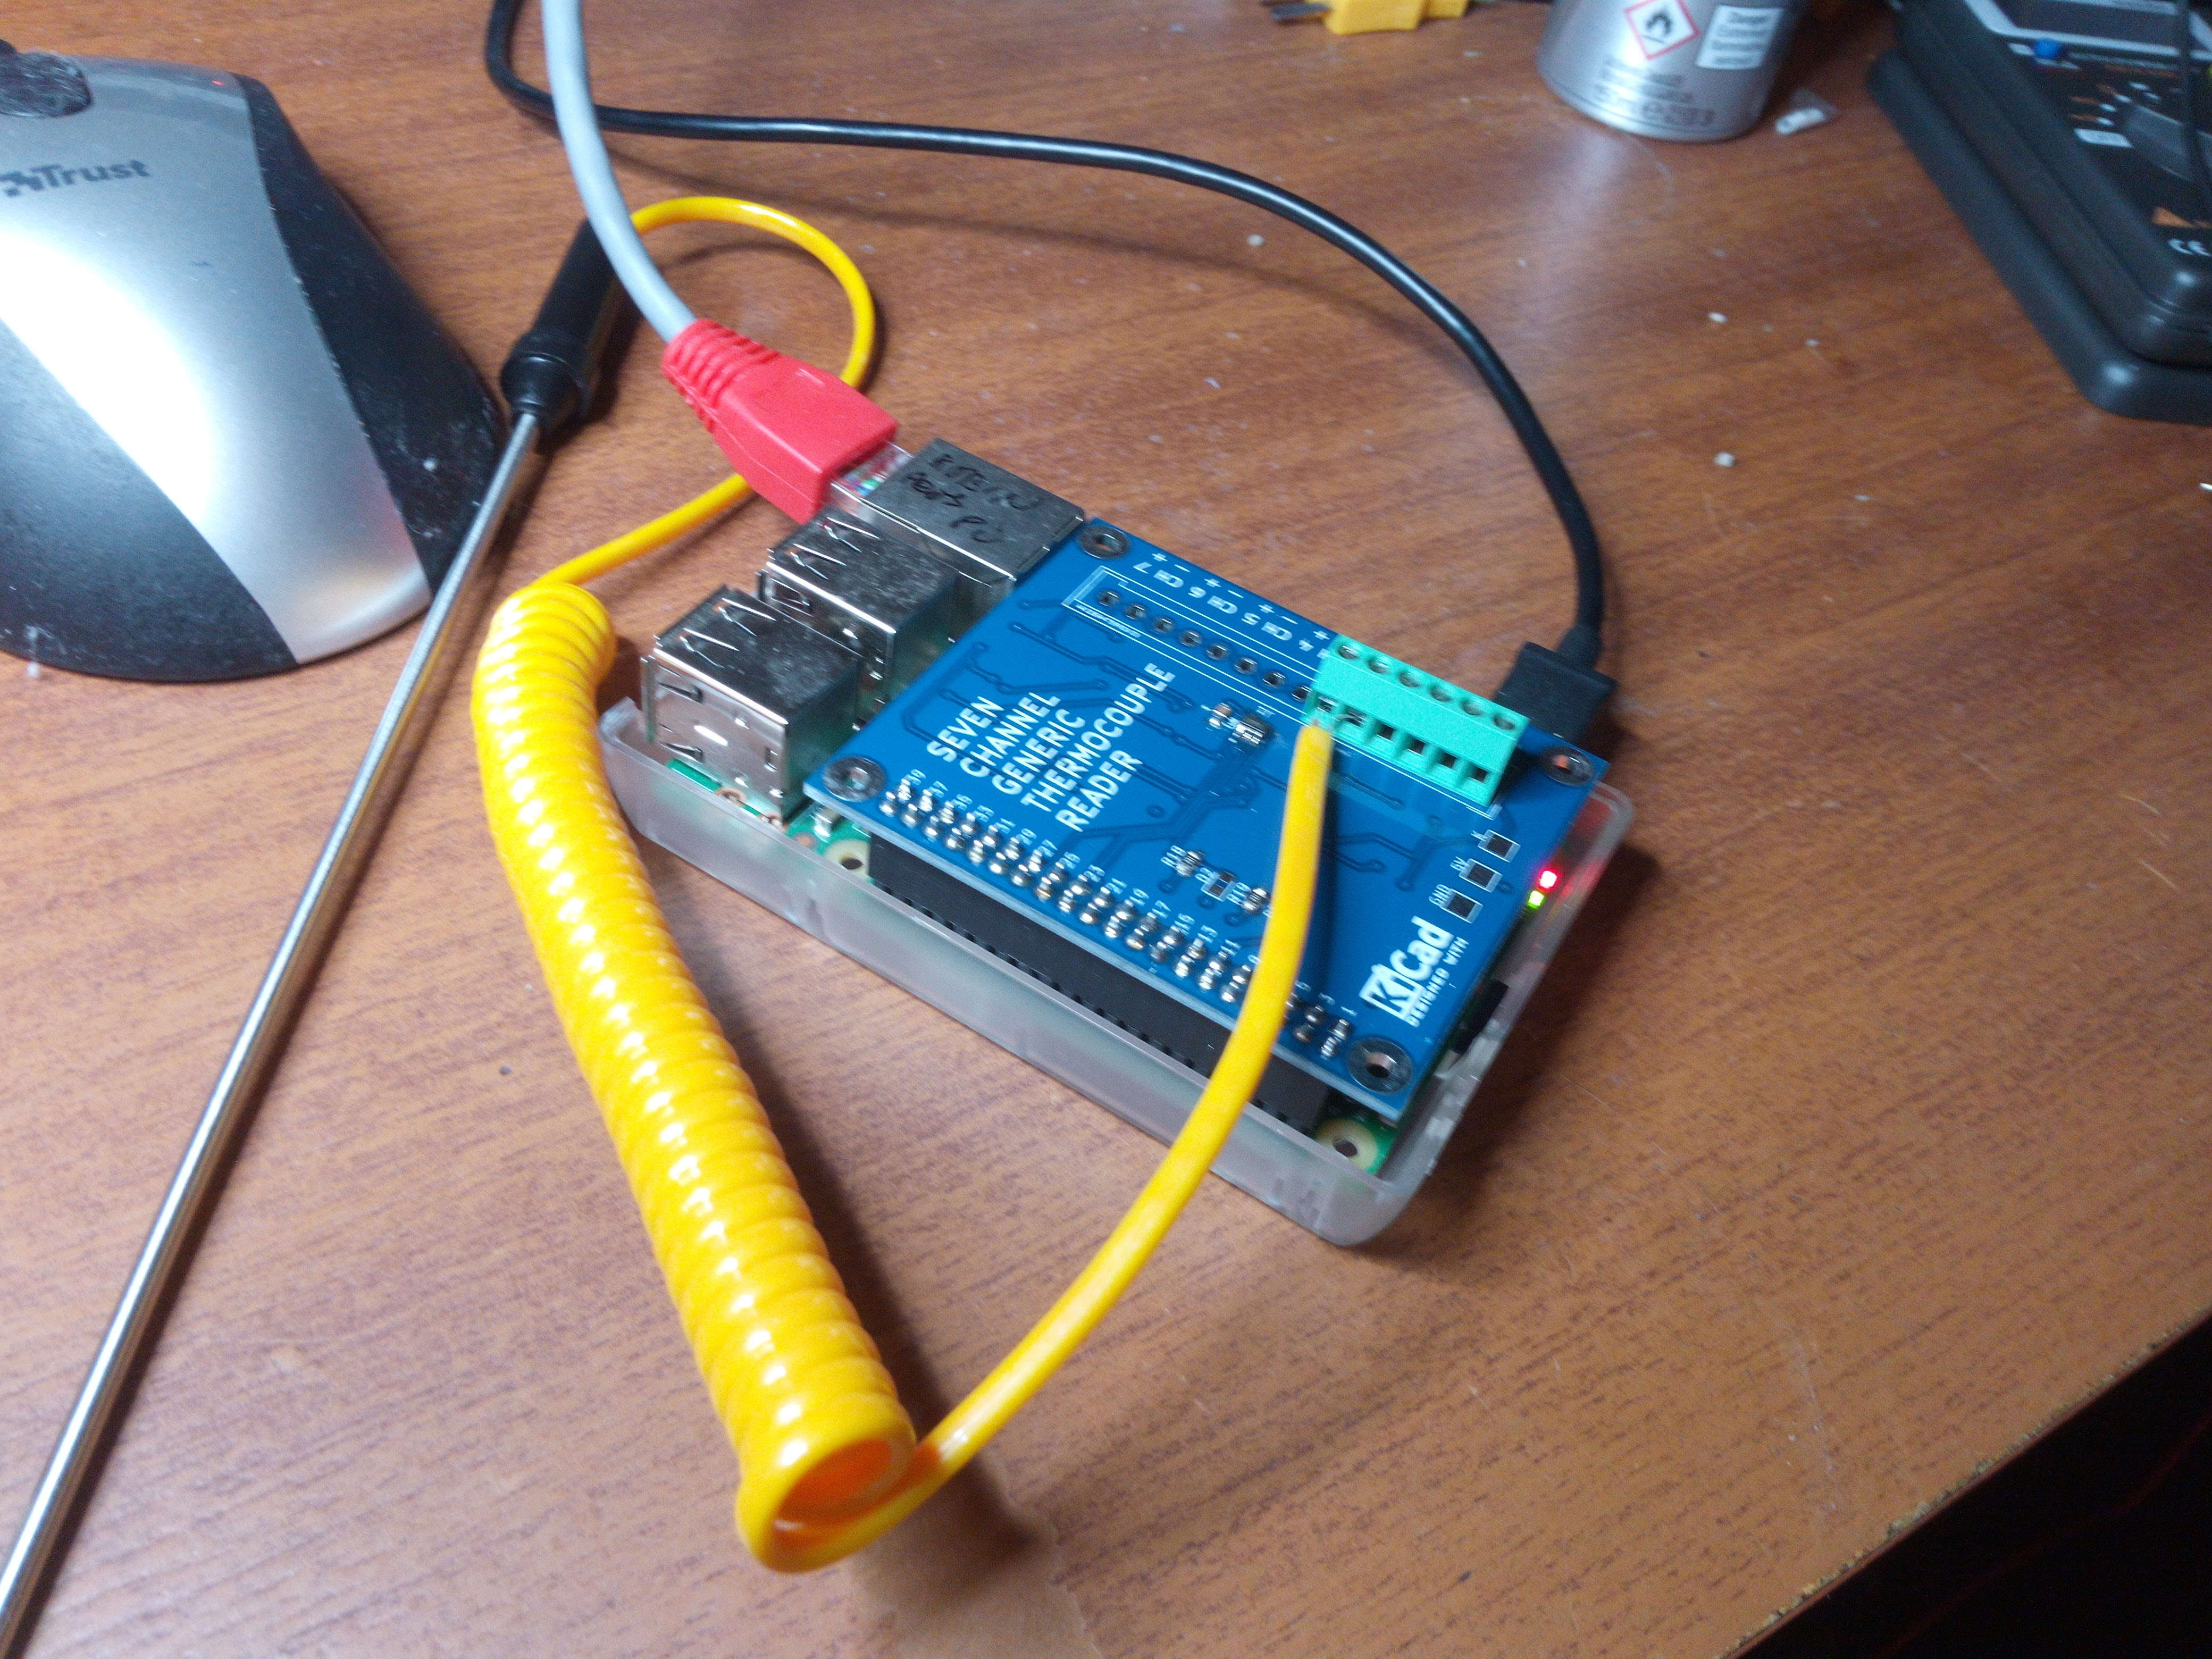
\includegraphics[width=200pt]{./TH7_0p4_IMG_20181010_184556D.jpg}
 % TH7_0p4_IMG_20181010_184556D.jpg: 0x0 pixel, 300dpi, 0.00x0.00 cm, bb=
 \caption{TH7 with a `k' type probe fitted.}
 \label{fig:th7}
\end{figure}



\section{TH7 Description}
%
The TH7 is a Raspberry~Pi hat   that
provides seven thermocouple inputs(see figure~\ref{fig:th7}).
%
This means seven different temperatures can be read
simultaneously. 
%
Its possible uses are 
logging/monitoring and control of temperature sensitive processes.
%
With on-board PCB temperature measurement, 
the PCB temperature
is used to implement
full Cold~Junction~Compensation (CJC).
%
Uncalibrated, the TH7 gives a typical accuracy of $\pm$ ${2}^{\circ} C$.
%
The TH7 also provides two user programmable LEDs; and 
makes available the PCB temperature, and the supply voltage to the Raspberry~Pi (USB voltage can vary between 4.7 to 5.2).
\clearpage
The TH7 is a generic thermocouple reader, and therefore should work with any thermocouple type.
%
Software defines its micro-volt to temperature and CJC characteristics.
Software support has currently only been written for the `k' type.

%\clearpage
\subsection{Characteristics}
The TH7 offers:
\begin{itemize}
 \item Full cold junction compensation;
 \item Thermocouple disconnection or open-circuit  detection;
 \item Seven inputs;
 \item Uses the Rasberry~Pi standard python SPI interface;
 %\item Python coding examples \\ https://github.com/robin48gx/TH7;
 \item Two user programmable LEDs;
 \item On chip PCB temperature measurement;
  \item Can be used as a general-purpose micro-volt 
  reader with a range of $\approx -6000 \mu V \rightarrow 40000 \mu V$.
\end{itemize} 

\section{Instructions}
\subsection{Connection to terminal block}
%
Connect the thermocouples using the hital~tech connectors and ensure the wires make contact with the 
connector metal clamps (see figure~\ref{fig:con}).
%
\subsection{Conection to the device being measured}
%
Always apply insulation to the thermocouples (i.e. do not ground them).
%
Epoxy resin is often useful for gluing thermocouples to devices under long term temperature tests.

\begin{figure}[h]
 \centering
 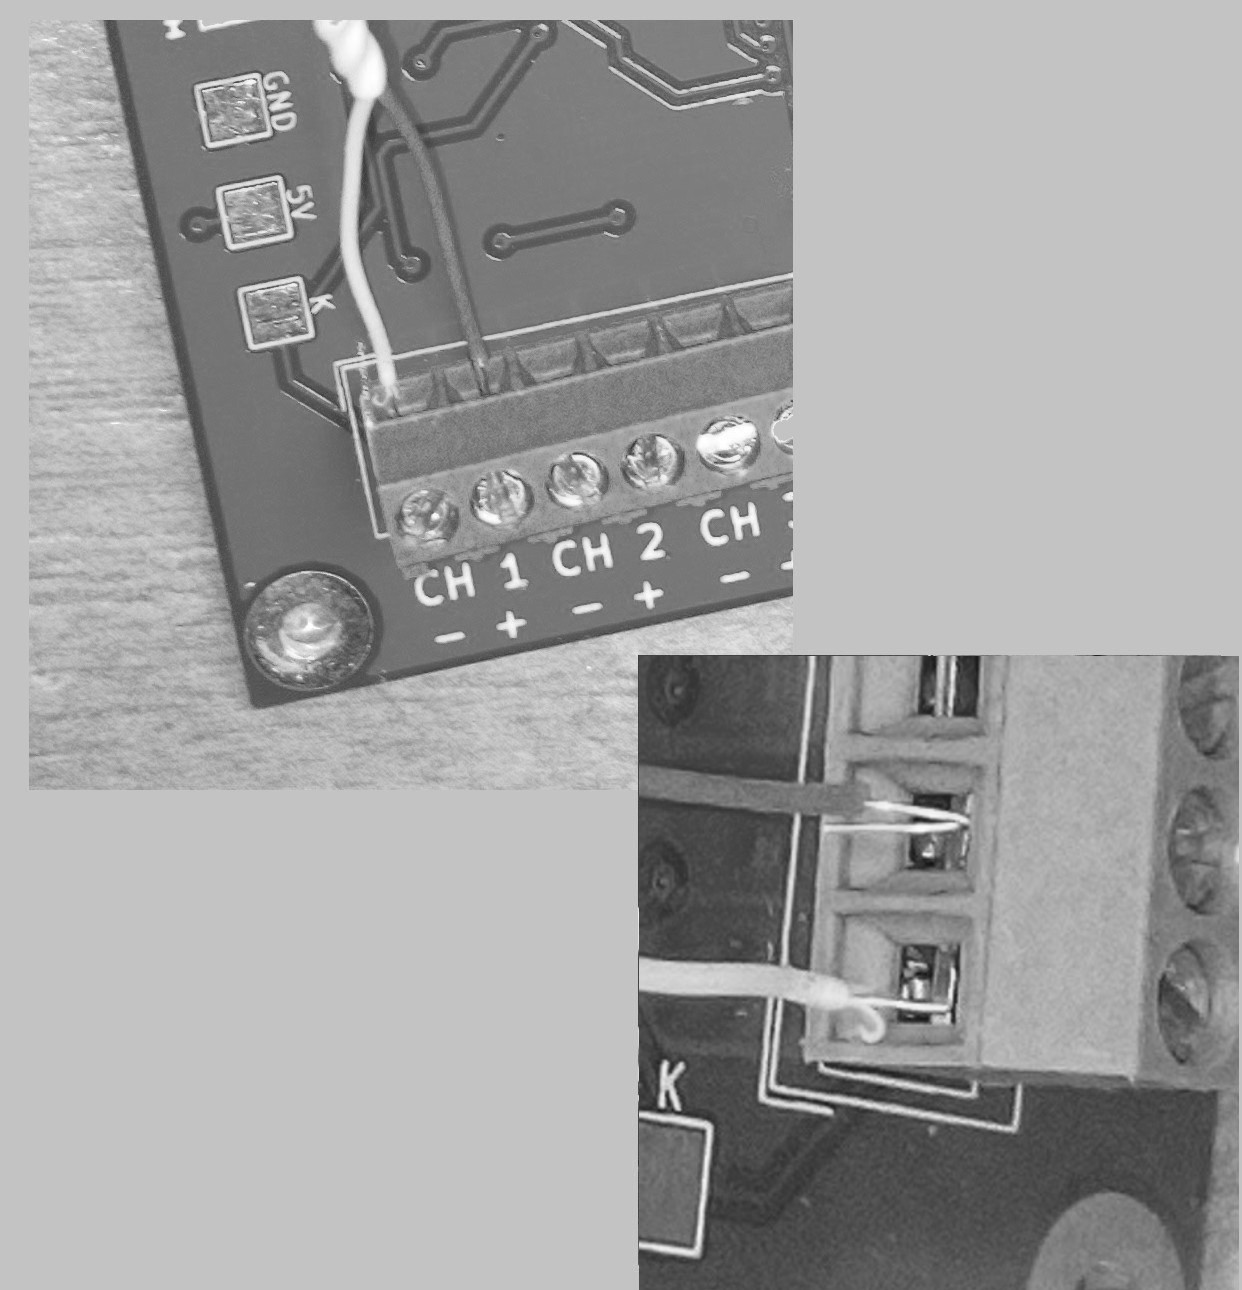
\includegraphics[width=200pt]{./wiring.jpg}
 % wiring.JPG: 0x0 pixel, 300dpi, 0.00x0.00 cm, bb=
 \caption{Image shows wiring for European standard `k' type thermocouples wiring (green is plus and the white is minus; other countries may use different colour schemes.)
%
 If the thermocouple is inserted with incorrect polarity it will read incorrectly and temperature will be seen to go down when heat is applied.}
 \label{fig:con}
\end{figure}

\begin{figure}[h]
 \centering
 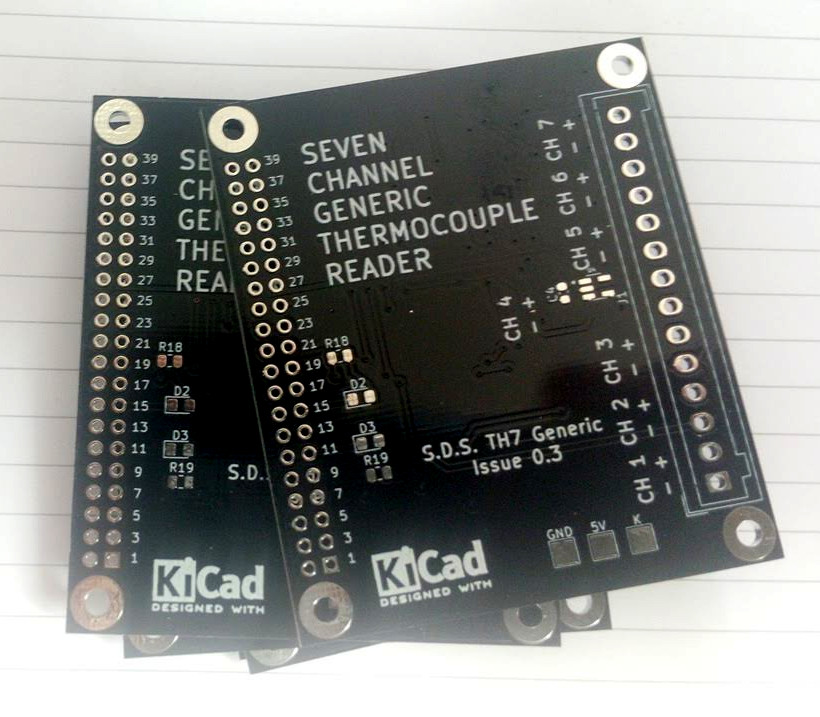
\includegraphics[width=156pt]{./TH7_0p3.jpg}
 % TH7_0p3.jpg: 0x0 pixel, 300dpi, 0.00x0.00 cm, bb=
 \caption{TH7 thermocouple Interface PCB/Raspberry~Pi~Hat}
 \label{fig:th7_2}
\end{figure}

\clearpage
\begin{figure}[ht]
 \centering
 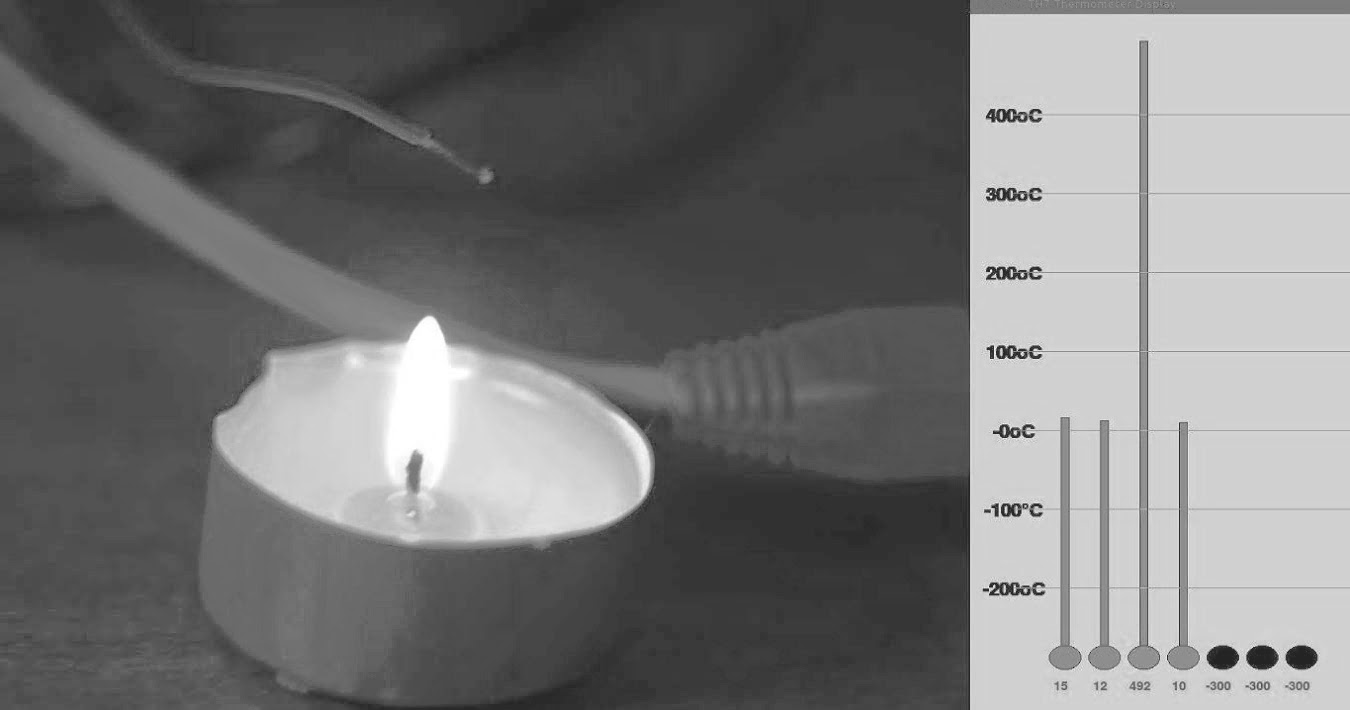
\includegraphics[width=200pt]{TH7_tea_light.jpg}
 % TH7_tea_light.JPG: 0x0 pixel, 300dpi, 0.00x0.00 cm, bb=
 \caption{Thermocouple over a tea light flame at circa ${500}^{\circ} C$.}
 \label{fig:pi}
\end{figure}
\mbox{}
\\
\\
\qrcode[height=1in]{http://www.scientificdatasystems.co.uk}
\\
\\
\vspace{0.5cm}
Contact: info@scientificdatasystems.co.uk
\\
\\
\qrcode[height=1in]{https://www.youtube.com/watch?v=EcGQWLSwX3U}
\\
\\
Youtube tutorial:
\\
https://www.youtube.com/watch?v=EcGQWLSwX3U
\vspace{0.5cm}
\clearpage

\section{What thermocouples are}

Thermocouples are two different types of metal wire welded together
at one end.
%
When there is a heat difference between two ends of the wire,
the two metals produce a small voltage.
%
This is typically very small, for `k' type thermocouples for instance,
this is about 40 millionths of a Volt per Centigrade change in temperature.
%
This voltage is so small that ordinary voltage reading chips, Analogue to Digital Converters (ADC),  cannot easily read them
to any reasonable accuracy.
%
The small signal is usually amplified
into a range that a computer chip (i.e. ADC) can read.
%
The TH7 has an amplifier that takes the small voltage and amplifies it by 100.
%
It can then be read into the Raspberry~Pi where it can be converted to
a temperature reading with adequate accuracy.
%
Wikipedia has a good entry on thermocouples.
https://en.wikipedia.org/wiki/Thermocouple.
%as a qrcode, \qrcode[height=1in]{https://en.wikipedia.org/wiki/Thermocouple}

\subsection{Cold Junction Compensation}

The tables and equations to convert thermocouple voltage to
temperature all assume that the instrument end is at zero centigrade.

Because the voltage read at the TH7 input is not at zero centigrade (well not normally!)
the junction of the wires {\em at the connector block}  makes a thermocouple itself, but in opposition to
the one at the measurement end.
%
For instance, with a `k' type thermocouple
the voltage read at $25^\circ C$ would read around $1000 \mu V$ low!

The TH7 has a temperature measurement chip placed right by the terminal block for the thermocouple inputs.
By knowing this temperature, the TH7 works out what the missing voltage is
and adds it in before calculating the final temperature. This is commonly known as cold junction compensation.

\subsection{Using the TH7 as a micro-volt reader}

The TH7 can be used as a general purpose micro-volt reader.
The voltage source must be floating i.e. not grounded.
A range of $\approx -6mV \rightarrow 40mV$ can be read.
\clearpage
\subsection{Availability}

TH7 boards are currently available with a four week lead time.
\\
\\
The TH7 is compatible with the Raspberry~Pi models 3 and 4.
\\
\\
TH7 boards may be customised for any thermocouple type.
An example for `k' type may be found on GITHUB 
\\
\\
\\
https://github.com/robin48gx/TH7 
\\
\\
\qrcode{https://github.com/robin48gx/TH7}
%\vspace{3.5cm}
%\clearpage
%\mbox{}
%\vfill
%\qrcode[height=1in]{http://www.scientificdatasystems.co.uk}
%\vspace{0.5cm}
\\
\\
\\
Contact: info@scientificdatasystems.co.uk
\\
\\
\qrcode[height=1in]{http://www.scientificdatasystems.co.uk}
\vspace{0.5cm}



\end{document}
